\subsection{INRIA contributions to dissemination}

Short summary:\\
$\circ$ 11 publications: 4 journals, 4 conference papers, 3 workshop papers\\
$\circ$ 2 international workshops: ICRA 2015 and BMVA 2015\\
$\circ$ 1 special issue organization in Autonomous Robots\\
$\circ$ dissemination of activies in several media



\subsubsection{Invited talks}

\begin{enumerate}
\item  Ivaldi, S. (12/2015) Human-robot interaction with iCub. Invited talk at University of Plymouth, by Samantha Adams and Angelo Cangelosi.
\item Ivaldi, S. (10/2015) Social and physical interaction with the iCub robot. Invited talk at Technical University of Munich (TUM) by Karinne Ramirez and Gordon Cheng.

\end{enumerate}

%\subsubsection{International events participation}
%
%\begin{enumerate}
%
%\item  Event ...
%
%\item  Event ...
%
%\end{enumerate}

\subsubsection{International events organization}

Organization of international Workshops:

\begin{enumerate}
\item  BMVA Workshop on Visual, tactile and force sensing for robot manipulation, December 9th 2015, London (UK), organized by L. Jamone and S. Ivaldi  (\url{http://www.eventbrite.co.uk/e/bmva-workshop-on-visual-tactile-and-force-sensing-for-robot-manipulation-registration-16836320889}). The workshop was sold out (more than 80 participants).

\item ICRA 2015 Workshop ICRA 2015 Workshop ``Get in touch! Tactile \& force sensing for autonomous, compliant, intelligent robots'', May 30th 2015, Seattle (USA), organized by S. Ivaldi, L. Jamone and B. Siciliano (\url{http://www.ausy.tu-darmstadt.de/Workshops/ICRA2015TactileForce}). The workshop had 147 registered participants.
\end{enumerate}



\subsubsection{Other events}

$\circ$ INRIA invited F. Nori (IIT) for a one-month research visit between January/February 2016. \\
$\circ$ S. Ivaldi (INRIA) participated to the iCub Summer School (VVV15) with the CoDyCo team. 
%
%\begin{enumerate}
%
%\item  Event ...
%
%\item  Event ...
%
%\end{enumerate}


\subsubsection{Talks at international conferences}

\begin{enumerate}
\item  Ivaldi, S. (2015) Social and physical interaction between humans and robots - perspectives for personal robotics assistants. Invited talk at NETT Workshop 2015 - Neural Engineering and related fields. Nancy, France.

\item Ivaldi, S. (2015) Multimodal object learning with iCub. BMVA Workshop on Visual, tactile and force sensing for robot manipulation, December 9th, London, UK.

\item Ivaldi, S. (2015) Individual differences and social signals during a human-robot assembly task. Workshop on Human-Friendly robotics, October 22th, Munich, Germany.
\end{enumerate}






\subsubsection{Editorial work}

S. Ivaldi (INRIA), together with J. Babic (JSI) and M. Mistry (UB), was guest editor for the journal Autonomous Robots (Springer) for the special issue on Whole-body control of contacts and dynamics for humanoid robots.

The CoDyCo project is explicitly mentioned in the editorial article. A dedicated page is also on the CoDyCo website (\url{https://www.codyco.eu/2-default/48-special-issue-auro}).


\subsubsection{Publications}

\begin{enumerate}

\item[Journals]

\item Ivaldi, S.; Babic, J.; Mistry, M.; Murphy, R. (2016) Special Issue on Whole-body control of contacts and dynamics for humanoid robots. Autonomous Robots, vol. 40, n.3, pp. 425-428. 

\item Lyubova, N.; Ivaldi, S.; Filliat, D. (2016) From passive to interactive object learning and recognition through self-identification on a humanoid robot. Autonomous Robots, vol. 40, n. 1, pp. 33-57. 

\item Anzalone, S.; Boucenna, S.; Ivaldi, S.; Chetouani, M. (2015) Evaluating the engagement with social robots. International Journal of Social Robotics, vol. 7, n. 4, pp. 465-478. 

\item Andries, M.;  Simonin, O.;  Charpillet, F. (2015) Localisation of humans, objects and robots interacting on load-sensing floors. IEEE Sensors Journal, Institute of Electrical and Electronics Engineers, PP (99), pp.12.

\item[Conferences]

\item Modugno, V.; Neumann, G.; Rueckert, E.; Oriolo, G.; Peters, J.; Ivaldi, S. (2016) Learning soft task priorities for control of redundant robots. Proc. IEEE International Conf. on Robotics and Automation (ICRA). 

\item Calandra, C.; Ivaldi, S.; Deisenroth, M.P.; Peters, J. (2015) Learning Torque Control in Presence of Contacts using Tactile Sensing from Robot Skin. International Conf. on Humanoid Robots (HUMANOIDS).

\item Calandra, R.; Ivaldi, S.; Deisenroth, M.P.; Rueckert, E.; Peters, J. (2015). Learning Inverse Dynamics Models with Contacts, Proc. IEEE International Conference on Robotics and Automation (ICRA). 

\item Traversaro, S.; Del Prete, A.; Ivaldi, S.; Nori, F. (2015). Inertial Parameters Identification and Joint Torques Estimation with Proximal Force/torque Sensing, Proc. IEEE International Conference on Robotics and Automation (ICRA). 

\item[Workshops]

\item Ivaldi, S.; Peters, J.;  Chetouani, M.;  Lefort, S.; Zibetti, E.; Provasi. J. (2015). Individual differences and social signals during a human-robot assembly task. Proceedings of the 8th International Workshop on Human-Friendly Robotics - HFR 2015, p. 40.

\item Modugno, V.; Neumann, G.; Rueckert, E.; Oriolo, G.; Peters, J.; Ivaldi, S. (2016) Learning soft task priorities for control of redundant robots. Proceedings of the 8th International Workshop on Human-Friendly Robotics - HFR 2015, p. 39.

\item Calandra, R.; Ivaldi, S.; Deisenroth, M.P.; Rueckert, E.; Peters, J. (2015) Learning Dynamics Models of Contacts from Tactile Sensors. Proceedings of the ICRA 2015 Workshop on Force and tactile sensing.

\item[Preprints]

\item Ivaldi, S.; Lefort, S.; Peters, J.; Chetouani M.; Provasi, J.; Zibetti, E. Towards engagement models that consider individual factors in HRI: on the relation of extroversion and negative attitude towards robots to gaze and speech during a human-robot assembly task. Preprint at arXiv:1508.04603 [cs.RO]. 

\end{enumerate}


	
\subsubsection{Media coverage}

\begin{figure}[!t]
\begin{center}
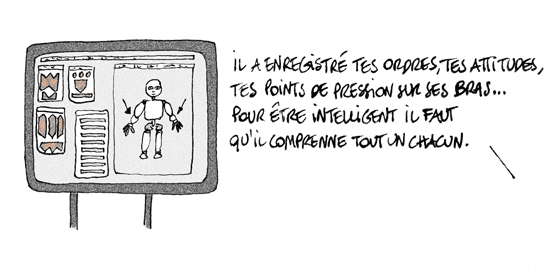
\includegraphics[height=4cm]{images/comic_fiamma_1.jpg}
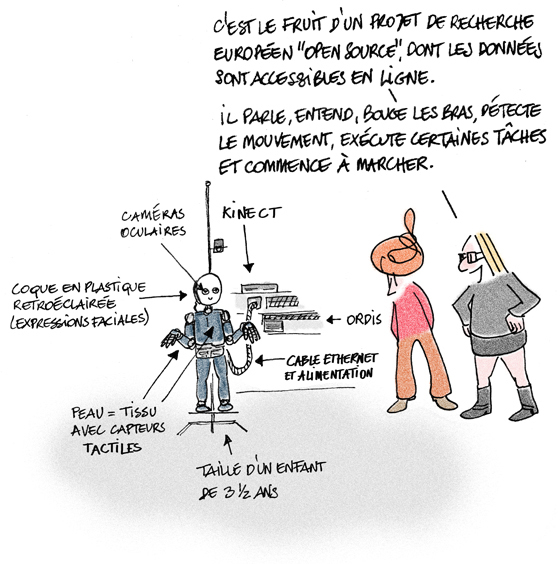
\includegraphics[height=4cm]{images/comic_fiamma_2.jpg}
\caption{Samples from the comic of Fiamma Luzzati describing the physical human-robot interaction experiments with the iCub (INRIA/UPMC).}
\label{fig:comicfiamma}
\end{center}
\end{figure}

\begin{itemize}

\item The CoDyCo experiments of human-robot physical interaction (collaboration INRIA \& UPMC) are portrayed by Fiamma Luzzati in her web article on Le Monde (\url{http://lavventura.blog.lemonde.fr/2014/04/07/qui-a-peur-du-robot-google/}), then in her book ``Le cerveau fait-il deux choses \`a la meme fois?'', Editions Delcourt (see Figure \ref{fig:comicfiamma}).
% (\url{http://www.editions-delcourt.fr/serie/cerveau-peut-il-faire-deux-choses-a-la-fois-et-autres-petites-questions-de-grande-importanc.html}).
\item Article in New Scientist, 21/10/2015 %\url{https://www.newscientist.com/article/mg22830442-300-what-will-it-take-for-humans-to-take-advice-from-a-robot/}
\item Article in Cit\'e Science, 29/10/2015
% (\url{http://www.cite-sciences.fr/fr/ressources/science-actualites/detail/news/peut-on-faire-confiance-aux-robots/?tx_news_pi1\%5Bcontroller\%5D=News&tx_news_pi1\%5Baction\%5D=detail&cHash=2edaeb3aeb42b9fc130afe5b02e9fab4})
\item Podcast interview for Interstices, 30/3/2016
% (\url{https://interstices.info/jcms/p_88305/des-robots-au-service-des-hommes?utm_content=bufferbb04b&utm_medium=social&utm_source=twitter.com&utm_campaign=buffer})
\item Article in La Semaine, 21/03/2016 
%(\url{http://www.lasemaine.fr/2016/03/17/tetes-chercheuses})
\item Article in Science et Vie Junior, 02/2016
\item Article in Pour la Science, 03/2016 
%(\url{http://www.pourlascience.fr/ewb_pages/a/article-les-robots-peuvent-ils-avoir-des-emotions-36560.php})

\end{itemize}
